In addition to shared-memory parallelism, the performance characteristics of the
MPI LES in a distributed-memory environment are of interest. The ability to run
on large computing clusters allows researchers using the LES to simulate at even
higher resolution or over larger areas than on a single machine.

Results were obtained using the EPSRC funded ARCHIE-WeSt High Performance
Computer (\url{www.archie-west.ac.uk}). EPSRC grant no. EP/K000586/1.

Each node on ARCHIE-WeSt has two Intel Xeon X5650 CPUs. This gives each node 12
cores running at 2.66GHz base frequency. The cluster was setup such that
hyperthreading was disabled but turbo boost was enabled. Each node is fitted
with 48GB RAM and nodes are connected to each other via a 4xQDR Infiniband
Interconnect. ARCHIE's MPI communication library was OpenMPI 1.6.2.

Even though the Intel CPUs have turbo boost enabled, all parallel runs use all
cores of the cluster so the frequency between runs is consistent.

\begin{figure}
    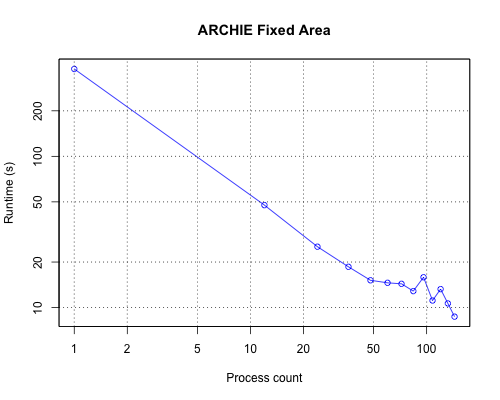
\includegraphics[width=0.5\textwidth]{graphs/ARCHIE-fixed-area.png}
    \caption{ARCHIE Fixed Area}
    \label{fig:archiefixedarea}
\end{figure}

Figure~\ref{fig:archiefixedarea} shows the performance scaling of a fixed area
problem over 12 nodes (144 cores). For 4 nodes (48 cores) there is good scaling
with 5 to 12 nodes offering only moderate improvements. The single process run
completes in 378.3 seconds. The 4 node run completes in 15.1 seconds and the 12
node run completes in 8.7 seconds. The first 48 cores offer a 25x improvement in
performance with the 144 core run offering a 43.5x improvement. This is expected
as the problem of less useful work per process and increasing communication
costs will ultimately become too great to overcome.

\begin{figure}
    \includegraphics[width=0.5\textwidth]{graphs/ARCHIE-expanding-area.png}
    \caption{ARCHIE Expanding Area}
    \label{fig:archieexpandingarea}
\end{figure}

Figure~\ref{fig:archieexpandingarea} shows the performance scaling of an
expanding area problem over 12 nodes (144 cores). The single core run takes
163.9 seconds. The single node (12 core) run takes 215.5 seconds and the 12 node
run takes 208.9 seconds. The variation in runtime between nodes is likely due to
the differing load on the cluster overall. Multiple runs of the 12 node run had
performance vary between 207 and 230 seconds. This gives an MPI overhead of
around 26.3 to 31.4\%. Crucially, the runtime does not grow on increasing node
count showing the strong scaling characteristics of the MPI LES.
